\svnidlong
{$HeadURL$}
{$LastChangedDate$}
{$LastChangedRevision$}
{$LastChangedBy$}
\svnid{$Id$}

Many different theories predict final states with a single top and associated missing 
transverse momentum (monotop), some of them including dark matter candidates. 
A simplified model encompassing the processes leading to this phenomenology is described in Refs.~\cite{AndreaFuksMaltoni,Agram:2013wda,Boucheneb:2014wza},
and is adopted as one of the benchmarks for Run 2 LHC searches. 

The simplified model is constructed by imposing that the model Lagrangian
respects the electroweak $SU(2)_L \times U(1)_Y$ gauge symmetry and by
requiring minimality in terms of new states to supplement to the Standard
Model fields. As a result, two monotop production mechanisms are possible.
In the first case, the monotop system is constituted by an invisible (or
long-lived with respect to detector distances) fermion $\chi$ and a top quark.
It is produced, as shown in the diagram of \ref{fig:feyn_prod}~(a) where a colored
resonance $\varphi$ lying in the triplet representation of $SU(3)_C$ decays
into a top quark and a $\chi$ particle. In the second production mode, the
monotop state is made of a top quark and a vector state $V$ connected to a
hidden sector so that it could decay invisibly into, e.g., a pair of dark
matter particles as studied in~\cite{Boucheneb:2014wza}. The production proceeds via
flavor-changing neutral interactions of the top quark with a quark of the
first or second generation and the invisible $V$ boson (see the diagrams of
\ref{fig:feyn_prod}~(b) and (c)).

%A dark matter candidate \chiDM and a new particle (vector or scalar) 
%are added to the SM, in a theory that respects the $\SUtwoUone$ symmetry 
%and produces a single top quark in association with either the DM particle or a new particle
%decaying invisibly. 

%Within this model, two distinct processes can lead to monotop production:
%\begin{itemize}
%	\item resonant production, as shown in the diagram of Fig.~\ref{fig:feyn_prod} (a), where a color triplet scalar $\varphi$ or vector field are exchanged in the \schannel, and decay into a spin 1/2 invisible new fermion $\chiDM$ and a top quark;
%	\item non-resonant production, as shown in the diagrams of Fig.~~\ref{fig:feyn_prod} (b) and (c), where a flavor-changing interaction produces a top quark in association with a new colored scalar or vector $V$. The new particles decay invisibly, e.g. to a pair of DM particles. $V$ can also decay into a top quark and an up quark, leading to a same-sign top quark final state; a detailed study of the complementarity of this signature is beyond the scope of this Forum report.  
%\end{itemize}

\begin{figure}[!h!tpd]
\centering
\unitlength=0.0046\textwidth
\subfloat[\label{subfig:S1}]{
  \begin{feynmandiagram}[modelS1]
    \fmfleft{i1,i2}
    \fmfright{o1,o2}
    \fmf{dashes,label={\Large $\varphi$}}{v1,v2}
    \fmf{fermion}{i2,v1,i1}
    \fmf{fermion}{v2,o1}
    \fmf{plain,tension=0}{v2,o2}
    \fmf{wiggly}{v2,o2}
    \fmfdot{v1,v2}
    \fmflabel{\Large ${\bar{s}}$}{i1}
    \fmflabel{\Large ${d}$}{i2}
    \fmflabel{\Large ${t}$}{o1}
    \fmflabel{\Large ${\chiDM}$}{o2}
  \end{feynmandiagram}
}\\\vspace{\baselineskip}
\subfloat[\label{subfig:S4s}]{
  \begin{feynmandiagram}[modelS4s]
    \fmfleft{i1,i2}
    \fmfright{o1,o2}
    \fmf{fermion,label={\LARGE $u$}}{v1,v2}
    \fmf{gluon}{i2,v1}
    \fmflabel{\LARGE $g$}{i2}
    \fmf{fermion}{i1,v1}
    \fmflabel{\LARGE $u$}{i1}
    \fmf{wiggly}{v2,o2}
    \fmf{fermion}{v2,o1}
    \fmflabel{\Large $V$}{o2}
    \fmflabel{\Large $t$}{o1}
  \end{feynmandiagram}
}
\subfloat[\label{subfig:S4t}]{
  \begin{feynmandiagram}[modelS4t]
    \fmfleft{i1,i2}
    \fmfright{o1,o2}
    \fmf{fermion}{i2,vup}
    \fmflabel{\LARGE $u$}{i2}
    \fmf{gluon}{i1,vdown}
    \fmflabel{\LARGE $g$}{i1}
    \fmf{fermion, label={\LARGE $t$}}{vup,vdown}
    \fmf{fermion}{vdown,o1}
    \fmflabel{\Large $t$}{o1}
    \fmf{wiggly}{vup,o2}
    \fmflabel{\Large $V$}{o2}
  \end{feynmandiagram}
  }
\caption
{
Feynman diagram of leading order processes leading to monotop events: production of
a coloured scalar resonance $\varphi$ decaying into a top quark and a spin-$1/2$ fermion $\chiDM$ (a),
$s-$ (b) and \tchannel (c) non resonant production of a top quark in association with
a spin-1 boson $V$ decaying invisibly.
%Feynman diagram of leading order processes leading to monotop events: resonant production of
%$t$ via resonant new particle $M$ decaying into a top quark and $\Xnew$, which is the dark matter fermion $\chiDM$ (left),
%and $s$ and $t$ channel non-resonant production of a top quark in association with $\Xnew$, which is the new particle $M$ (middle and right).
}
\label{fig:feyn_prod}
\end{figure}

%In the following, resonant and non-resonant production are treated independently as separate benchmarks. 
%Only the simpler case of a scalar resonance and the non-resonant vector are considered as early benchmarks 
%for the resonant model; the other two cases with a more complicated phenomenology can be studied in the future. 
%CD: why? the vector is better in "revisiting monotop"

\newthought{Resonant production}
\label{sec:ResonantProd}

In this case, a colored $2/3$-charged scalar ($\varphi$) is produced and decays into a top quark and a spin-$1/2$ invisible particle, $\chiDM$.  The dynamics of the new sector is described by the following Lagrangian:

\be\label{eq:lagrangianResonant}\bsp
\lag &=
%\lag_{\rm SM} + \lag_{\rm kin} 
%%
%+ 
\bigg[
%\phi \bar u \Big[a^0_{FC}\!+\!b^0_{FC} \gamma_5 \Big] u \!+\!
%V_\mu \bar u \gmu \Big[a^1_{FC} \!+\! b^1_{FC} \gamma_5 \Big] u  \\
%%
%&+ 
\varphi \bar d^c
\Big[a^q_{SR} + b^q_{SR} \gamma_5 \Big] d +
\varphi \bar u \Big[a^{1/2}_{SR} + b^{1/2}_{SR} \gamma_5 \Big] \chiDM
%
%\\ &
%+ X_\mu \bar d^c\gmu
%\Big[a^q_{VR} + b^q_{VR} \gamma_5 \Big] d
%%
%+ X_\mu \bar u \gmu
%\Big[a^{1/2}_{VR} + b^{1/2}_{VR} \gamma_5 \Big] \chiDM 
+ 
{\rm h.c.} \bigg] 
\esp\ee
%\begin{eqnarray}
%\label{eq:lagrangianResonant}
%\mathcal{L} =  d^{C}_{i} \:  [ (g^{v}_{\phi d})^{ij} +  (g^{a}_{\phi d})^{ij} \gamma^{5} ] \: d_{j} \: \phi^{\pm}  +  u^{C}_{k}  [ (g^{v}_{u\chiDM})^{k} + (g^{a}_{u\chiDM})^{k} \gamma^{5} ] \: \chiDM \: \phi^{\pm}
%%%CD: problems with the original typesetting
%\end{eqnarray}
where $u$ ($d$) stands for any up-type (down-type) quark, the notation $SR$
refers to the monotop production mechanism via a scalar resonance and all
flavor and color indices are understood for clarity.

%The first term leads to the production of the new particle and the last term allows its decay into a $up$-quark 
%and a non interacting fermion (in particular to the top quark when $(g^{v/a}_{u\chiDM})^{k}$ 
%is sizable mainly for $k=3$).
%This model is then described by the masses of the new particle $m_{\phi}$ and the invisible 
%fermion $m_{\chiDM}$, and the coupling 
%$(g^{v/a}_{\phi d})^{ij}$ and $(g^{v/a}_{u\chiDM})^{k}$.

In the notation of~\cite{Agram:2013wda}, 
the couplings of the new colored fields to down-type quarks are
embedded into the $3\times 3$ antisymmetric matrices
$a^q_{SR}$ (scalar couplings) and $b^q_{SR}$ (pseudoscalar couplings)
while those to the new fermion $\chiDM$ and one
single up-type quark are given by the three-component vectors
$a^{1/2}_{\{S\}R}$ and $b^{1/2}_{\{S\}R}$
in flavor space. 

% 
% \com{Question/comment: in this resonant model, this is not so obvious to interpret $\phi_{\pm}$ as the new particle since there is a vertex $\phi-u-\chiDM$.
% It is somehow breaking the concept of having a dark sector weakly coupled to ordinary matter via a new particle.}

  Under the form of Eq.~\eqref{eq:lagrangianResonant}, the Lagrangian corresponds to the one
  introduced in the original monotop search proposal~\cite{AndreaFuksMaltoni} and has been
  used by the CMS for Run I analyses after neglecting the pseudoscalar component
  of the coupling and adding the vector resonance case for which minimality
  requirements are difficult to accomodate~\cite{CMSmonotop}. In contrast, the
  study of  Ref.~\cite{Boucheneb:2014wza} has imposed electroweak gauge invariance and
  requires minimality, which enforces all new couplings to be right-handed,




Under the form of Eq.~\eqref{eq:lagrangianResonant}, the Lagrangian is the one
introduced in the original monotop search proposal~\cite{AndreaFuksMaltoni}. It has been
used by the CMS collaboration for Run I analyses after neglecting all pseudoscalar components
of the couplings and adding the vector resonance case for which minimality
requirements are difficult to accomodate~\cite{CMSmonotop}. In contrast, the
study of Ref.~\cite{Boucheneb:2014wza} has imposed electroweak gauge invariance and
required minimality. This enforces all new couplings to be right-handed so that
\begin{equation}
a^{1/2}_{SR} = b^{1/2}_{SR} = \frac12 y_s^*
\qquad\text{and}\qquad
a^q_{SR} = b^q_{SR} = \frac12 \lambda_s \ ,
\end{equation}
where the objects $\lambda_s$ and $y_s$ are
a tridimensional vector and a $3\times 3$ matrix
in flavor space respectively. 
This class of scenarios is the one that has been adopted by the ATLAS collaboration for its
Run~I monotop searches~\cite{ATLASmonotop} and will be considered by both
collaborations for Run~II analyses.

%In the following, we only consider the model with a new colored scalar, as the requirement of invariance
%under $SU(2)_L \times U(1)_Y$ would require the introduction of further particles in the case of a new colored vector~\cite{Boucheneb:2014wza}.
%Note that the resulting model can be likened to the MSSM with
%an RPV coupling between a top squark and fermions and an RPC coupling
%between a top squark--top--neutralino.

The resulting model can be likened to the MSSM with an $R$-parity violating of
a top squark to the Standard Model down-type quarks and an $R$-parity
conserving interaction of a top quark and a top-squark to a neutralino.
  

\newthought{Non-Resonant production}
\label{sec:NonResonantProd}

For non-resonant monotop production, the monotop state is produced via
flavor-changing neutral interactions of the top quark, a lighter up-type
quark and a new invisible vector particle $V$. 
This is the only case considered, as having a new scalar 
would involve a mixing with the SM Higgs boson and therefore a larger number of free parameters. 
The Lagrangian describing the
dynamics of this non-resonant monotop production case is:
%%CD: Full explanation is below
% First, the new particle can be a scalar field interacting with the SM field and the dark matter
% candidate as described in this lagrangian:
% \begin{equation}
%  \label{eq:lagrangianNonResonantScalar}
% \mathcal{L} =  u^{C}_{i} \:  [ (g^{v}_{\phi u})^{ij} +  (g^{a}_{\phi u})^{ij}  \gamma^{5} ] \: u_{j} \: \phi  
%  +  \chiDM^{C}  [ g^{v}_{\phi\chiDM} + g^{a}_{\phi\chiDM}  \gamma^{5} ] \chiDM \: \phi
% \end{equation}
% where $u$ stands for any $up$-quark, the index $v$ ($a$) stands for vectorial (axial), 
% $C$ means charge conjugate and $i,j,k$ run over the generations.
% The first term describes the interaction between the new particle and the $up$-quarks while the 
% second term leads to the decay of the new particle into invisible fermions. 
% In this model, there is necessarily a mixing between $\phi$ and  the Higgs boson field. 
% Additional parameters are then required to describe this new sector: in addition to 
% the new particle mass and couplings, the mixing matrix of the two scalar fields
% is needed in order to make predictions. For the sake of simplicity, 
% we do not consider this case were the parameters space would be too large.
\be\label{eq:lagrangianNonResonantVector}\bsp
\lag &=
%\lag_{\rm SM} + \lag_{\rm kin} 
%%
%+ 
\bigg[
%\phi \bar u \Big[a^0_{FC}\!+\!b^0_{FC} \gamma_5 \Big] u \!+\!
V_\mu \bar u \gmu \Big[a^1_{FC} \!+\! b^1_{FC} \gamma_5 \Big] u  
%
+ \rm h.c. 
\bigg] 
\esp\ee
where the flavor and color indices are
again understood for clarity.

The strength of the interactions among these two states and a pair
of up-type quarks is modeled via two $3\times 3$ matrices in flavor space $a^{\{1\}}_{FC}$ for the vector couplings
and $b^{\{1\}}_{FC}$ for the axial vector couplings.

%The dynamics of this case is described by the following Lagrangian:
%\begin{equation}
% \label{eq:lagrangianNonResonantVector}
%  \mathcal{L}  =  \bar{u}_{i} [ (g^{v}_{Vu})^{ij} \gamma^{\mu} + (g^{a}_{Vu})^{ij} \gamma^{5} ] u_{j} \: V_{\mu}  
%  +  \bar{\chiDM} [ g^{v}_{Vu} \gamma^{\mu} + g^{a}_{V\chiDM} \gamma^{5} ]   \chiDM \: V_{\mu}
%\end{equation}
%where $u$ stands for any $up$-quark, the index $v$ ($a$) stands for vectorial (axial) and $i,j,k$ run over the generations.
%The first term describes the interaction between the new particle and the $up$-quarks while the second term leads to the decay the new particle 
%into invisible fermions. The new sector can be defined with the couplings $(g^{v/a}_{Vu})^{ij}$, 
%$g^{a/v}_{V\chiDM}$ and the masses $m_V$ and $m_{\chiDM}$. 
%This model can be probed by two different experimental signatures: monotop and same-sign top quark production. 
%% 
%% \com{Question for theorists: why it cannot mix with $\Zboson$ in case of vectorial new particle ?}

As for the resonant case, the Lagrangian of Eq.~\eqref{eq:lagrangianNonResonantVector} is the one that
has been used by CMS after reintroducing the scalar option for the invisible
state and neglecting all pseudoscalar interactions~\cite{CMSmonotop}. as
already mentioned, a simplified setup motivated by gauge invariance and
minimality has been prefered so that, as shown in Ref.~\cite{Boucheneb:2014wza}, we
impose all interactions to involve right-handed quarks only in order to simplify the model phenomenology,
\begin{equation}
a^1_{FC} = b^1_{FC} = \frac12 a_R
\end{equation}
where $a_R$ denotes a $3\times 3$ matrix in flavor space.

\newthought{Model parameters and assumptions}
 
The models considered as benchmarks for the first LHC searches
contain further assumptions in terms of the flavour and chiral structure of the model
with respect to the full Lagrangians of equations~\eqref{eq:lagrangianResonant} and~\eqref{eq:lagrangianNonResonantVector}.

%We only consider right-handed quark components, in order to simplify the model phenomenology. 
%The representation of the left-handed components under the $\SUtwo$ symmetry would lead to a 
%coupling to $down$-type quarks, since the effective theory is invariant under $\SUtwoUone$ 
%gauge symmetry. 

%%Having a coupling between the new particle and $down$-type quarks 
%would complicate the collider phenomenology, adding the
%$V \to b\bar{d} + \bar{b}d$ decay mode in addition to the invisible decay mode. 
%This in turn sets the scalar (vector) and pseudoscalar (axial vector) matrices to have 
%elements of equal values. 
This implies the vector to be an SU(2)L singlet, hence in turn setting the vector and axial vector matrices 
to have elements of equal values. 

%Furthermore, in order to be visible at the LHC in the monotop final state, 
%these models must include a strong coupling between the new particle $\phi$ and $t\chiDM$.
%%In the resonant case, the new particle must also couple to light quarks in order
%%to be produced at the LHC, leading to possible constraints from
%%dijet searches. 
%The same kind of assumption exists for the non-resonant production. 
%This means that only the couplings between the new scalar resonance and  
%light quarks ($a_{VR}, a_{SR}$), and the couplings between the new vector, the top quark 
%and light quarks ($a_{FC}$), are set to non-zero values 
%\be\label{eq:a}\bsp
%%& (a^0_{FC})_{13} = (a^0_{FC})_{31} = a
%(a^1_{FC})_{13} = (a^1_{FC})_{31} = a \ , \\
%(a^q_{SR})_{11} = (a^{1/2}_{SR})_3 = a
%\esp 
%\ee

In order to have an observable monotop signature at the LHC, the Lagrangians
introduced above must include not too small couplings of the new particles to
first and second generation quarks. For simplicity, we assumed that only
channels enhanced by parton density effects will be considered, so that we fix
\begin{equation}\bsp
(a_R)_{13} = (a_R)_{31} = a \ , \\
(\lambda_s)_{12} = - (\lambda_s)_{21} = \lambda
\qquad\text{and}\qquad
(y_s)_3 = y \ ,
\esp\end{equation}
all other elements of the matrices and vectors above being set to zero.

\todo{There is still an on-going study that should be finished very soon (by the end
	of the week). The point is that CMS is fixing the $y$ parameters in the way that
	the branching ratio of the scalar resonance into a monotop system is close to
	100\%, while ATLAS is fixing y = lambda. We are investigating both cases so to
	conclude whether this is good to keep both options allowed.
	}
%  (on top of $V \to t\bar{u} + \bar{t}u$ and $V \to \chiDM\chiDM$). 
 
%
%Typically, including 
%the left-handed components of quarks in the lagrangian~\eqref{eq:lagrangianNonResonantVector} 
%describing the $Vtu$ vertex would lead to 
%\begin{equation}
%\mathcal{L}_{Vtu} \; = \;  g^{R}_{Vtu} \: \bar{t}_{R}\gamma^{\mu}u_R \: V_{\mu} \; + \; g^{L}_{Vtu} 
%(\bar{t}_{L}\gamma^{\mu}u_L \: + \:  \bar{b}_{L}\gamma^{\mu}d_L ) \: V_{\mu}
%\end{equation}
%where $g^{R/L} \equiv 1/2 \, (g^{v} \pm g^{a})$ couples only to right-handed/left-handed components. 
%The second term stems from invariance under $\SUtwo$ rotations, and leads to an additional 
%decay mode $V \to b\bar{d} + \bar{b}d$ (on top of $V \to t\bar{u} + \bar{t}u$ and $V \to \chiDM\chiDM$). 

%Given that the new particle must be produced from a light quark in the initial state, 
%in association with a top quark, the monotop signature can mainly probe a high 
%coupling $\left(g^{v/a}_{Vu}\right)^{13}_{Vu} \equiv g^{v/a}_{Vtu}$. 

%Therefore,
%the sensitivity to other flavour couplings is significantly lower, since $V$ would be 
%produced at a lower rate. 

%CD: not sure I understand?
% In addition, the new particle must decay into invisible particles
% to lead to the searched monotop final state. As a consequence, the sensitivity for 
% scenario where $\BR{V}{\chiDM\chiDM}\ll 100\%$ can be quite low. 
% To cope with this second limitation, a same-sign top quark final state 
% $gu \to tV(\to t\bar{u})$ is proposed to cover the cases where $V$ would decay
% into visible particles. This case is more likely as the $tV$ production rate increases, 
% and becomes then a key point to constraint this model in a consistent way.

% % \com{Questions for theorists:
% % \begin{itemize}
% %  \item How well these flavour assumptions are allowed by the other HEP data (proton decay life time, flavour physics, etc ...) ?
% %  \item MFV criteria ?
% % \end{itemize}
% % }
% 
% \subsubsection{Chiral structure}
% \label{sec:chiralstructure}

\newthought{Implementation}
The Monte Carlo simulation relevant for
this case is discussed in Appendix~\ref{app:MonojetLikeModels_Appendix}.


%In the case of the non-resonant model and . 
%Further studies will show whether to a top and an up quark 

%The two matrices $A$ and $B$ are taken to be equal according to the chiral assumptions made above. 
%The convention adopted follows \cite{ATLASmonotop} in defining 
%a single number $a_{\mathrm{res}}$ ($a_{\mathrm{non-res}}$) 
%for the resonant (non resonant) model, such as $(\ares^q)_{\mathrm{12}}=(\ares^q)_{\mathrm{21}}=(\ares^{1/2})_{\mathrm{3}}\equiv \ares$ 
%(in order to have $d-s-S$ couplings, and $t-S-f_{met}$ couplings) 
%and $(\anonres)_{\mathrm{13}}=(\anonres)_{\mathrm{31}}\equiv \anonres$ (in order to have $v_{met}-t-u$ couplings). 

\subsection{Parameter scan}

The relevant parameters for the resonant model are:
\begin{itemize}
	\item The mass of the new scalar $\phi$;
	\item The mass of the new fermion $\chiDM$;
	\item The coupling of the new scalar to the new fermion and top quark $a$, 
	related to the width of the scalar in the minimal width assumption;
\end{itemize}	

The relevant parameters for the non-resonant model are:
\begin{itemize}
	\item The mass of the new vector $V$;
	%\item The mass of the new fermion $\chiDM$;
	\item The coupling of the new vector to the up and top quark $a$, 
	related to the width of the scalar in the minimal width assumption;
	\item The coupling of the new vector to the new fermion $\chiDM$, 
	related to the branching fraction of the vector into invisible and visible particle,
	and as a consequence to the width of the vector. 
\end{itemize}	
%
%In the case of the non-resonant model, the current implementation
%of the model does not allow changing the new fermion mass directly 
%as it is not explicitly implemented. 

In the case of the non-resonant model, the invisible vector is connected to
a hidden sector that could be, in its simplest form, parameterized by a new
fermion. This has effects on the width of the invisible $V$ state.

It has been checked for the non-resonant model that the relevant kinematics 
does not change when changing 
the width of the resonance, for widths up to 10\% of the $V$ mass. 
Figures~\ref{fig:appB:Vmass} and \ref{fig:appB:pTV} show 
the $V$ mass distribution, the transverse momentum for $V$ 
%and for the top quark 
in the case of the $V\to t\bar{u}$ decay, for different $V$ masses and widths.
Since they only show kinematic quantities related to $V$, these figures are relevant independently of the $V$ decay mode (be it visible or invisible). 
\Todo{Pictures will be improved in the next drafts.}
\begin{figure}[!h!tpd]
	\centering
	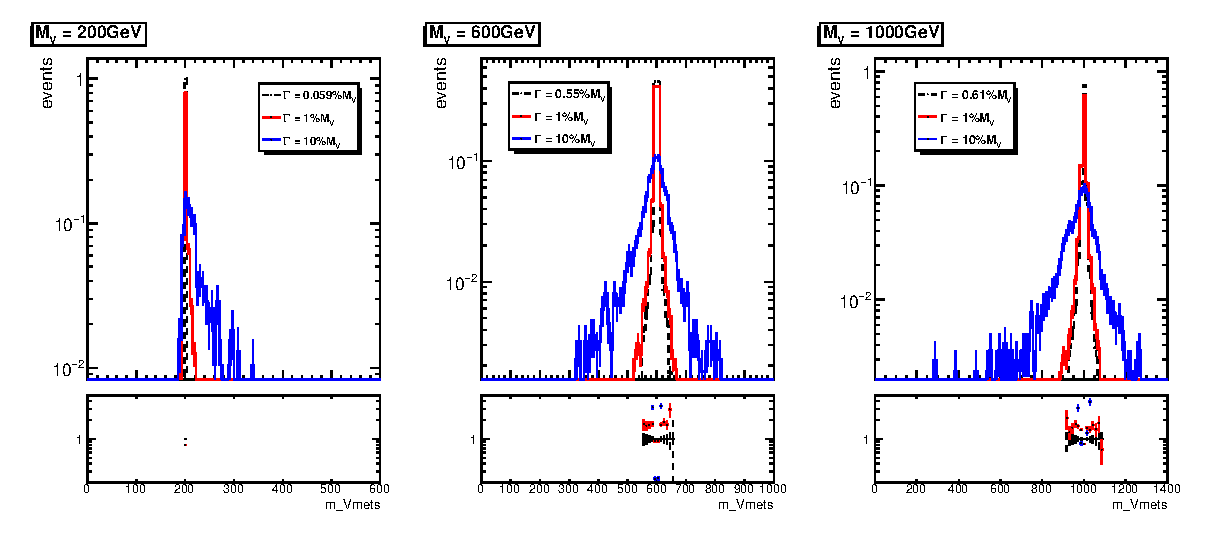
\includegraphics[width=1.0\textwidth]{figures/singletop/m_Vmets}
	\caption{
		Distribution of $V$ invariant mass for the $gu\to tV(\to t\bar{u})$ (on-shell V) 
		for $m_V$ = {200, 600, 1000}~GeV (from left to right) and for three different
		visible decay width (computed from \madgraph directly according to the allowed decays and their couplings, $1\%$ and $10\%$).
	}   
	\label{fig:appB:Vmass}
\end{figure}


\begin{figure}[!h!tpd]
	\centering
	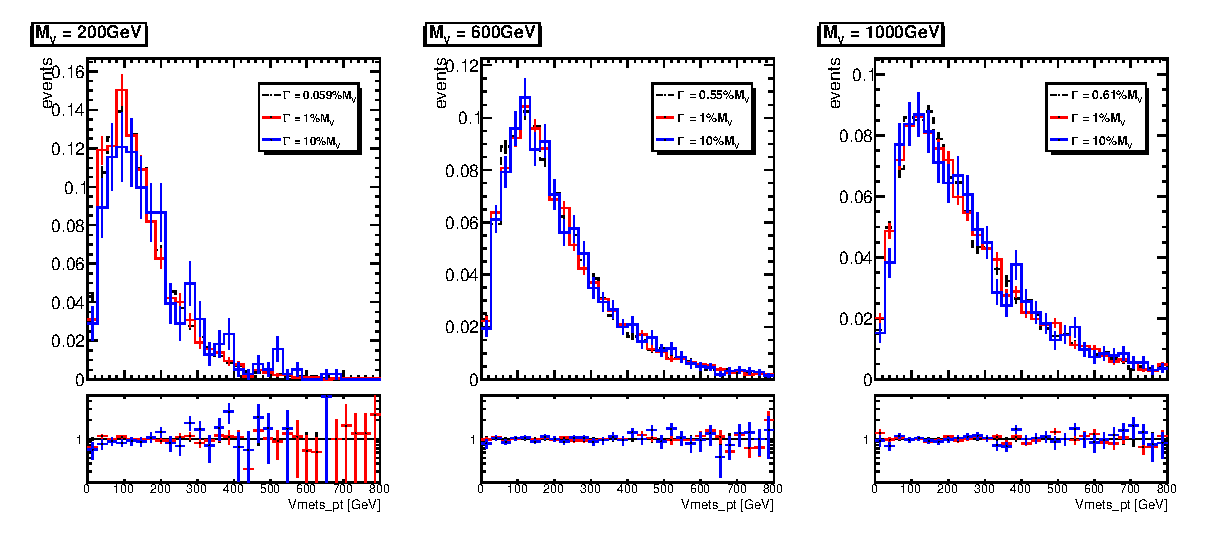
\includegraphics[width=1.0\textwidth]{figures/singletop/Vmets_pt}
	\caption{
		Distribution of the $V$ $p_T$ for the $gu\to tV(\to t\bar{u})$ (on-shell V) for $m_V$ = {200, 600, 1000}~GeV (from left to right) and for three different
		visible decay width (computed from \madgraph directly, $1\%$ and $10\%$).
	}
	\label{fig:appB:pTV}
\end{figure}


%\begin{figure}[!h!tpd]
%	\centering
%	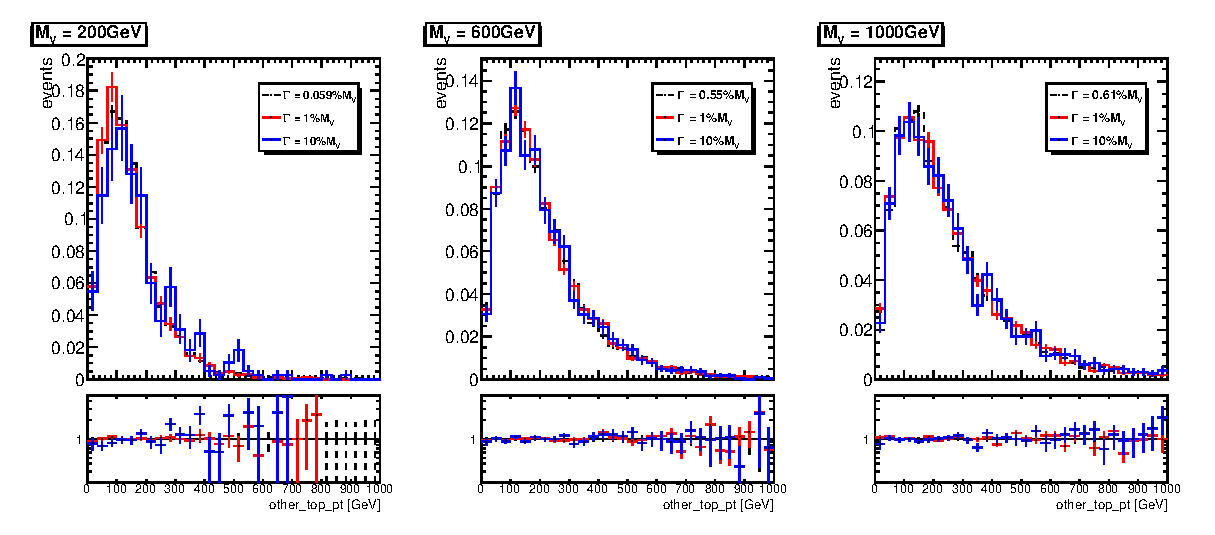
\includegraphics[width=1.0\textwidth]{figures/singletop/other_top_pt}
%	\caption{
%		Distribution of the top quark $p_T$ produced in association with $V$ in $gu\to tV$ for $m_V$ = {200, 600, 1000}~GeV (from left to right) and for three different
%		visible decay width (computed from \madgraph directly, $1\%$ and $10\%$).
%	}
%	\label{fig:appB:pTtop}
%\end{figure}

The limited timescale allowed to reach a consensus for
the recommendations contained in this document has not allowed further studies on the 
parameter scan of these models. The two Collaborations have however agreed to continue studying
these models and agree on a common parameter scan,
following the same path as for other models described in this document.  

%\newthought{Parameter choices and cross sections}
%
%\textbf{[Open point: update with new numbers]}
%
%ATLAS has considered two models, a resonant and a non-resonant production, using only right-handed top quarks in the lepton+jets final state. The signal samples were produced with \madgraph v1.5.11 interfaced with {\sc Pythia} 8.175, using the MSTW2008LO Parton Distribution Function (PDF) set (lhapdf ID: 21000).
%The mass of the top quark was set at 172.5 GeV. Dynamic renormalisation and factorisation scales were used.
%The $\met$ particle mass was varied, and in the case of the resonant model the resonance mass was fixed at 500~GeV:
%\begin{itemize}
%\item Resonant model,  $\met$ particle mass: [0,100]~GeV in 20~GeV steps
%\item Non-resonant model, $\met$ particle mass: [0,150]~GeV in 25~GeV steps, [200,300]~GeV in 50~GeV and [400,1000]~GeV in 100~GeV steps 
%\end{itemize}
%
%%\com{How to translate the monotop paper couplings to the notation of this note? }
%The couplings $\ares$ and $\anonres$ are set at a fixed value of $0.2$.
%In addition, two samples are produced for the resonant model for $\mfmet=100$~GeV,
%with coupling strengths fixed at $\ares=0.5$ and $\ares=1.0$,
%in order to check the effect of the resonance width on the signal event kinematics. 
%The total width of the resonance varies quadratically with the coupling strength,
%corresponding to a width of 3.5~GeV, 21.6~GeV, and 86.5~GeV at $\ares=0.2$, $\ares=0.5$, and $\ares=1.0$, respectively.
%
%The number of free parameters is reduced by assuming $(\ares^q)_{\mathrm{12}}=(\ares^q)_{\mathrm{21}}=(\ares^{1/2})_{\mathrm{3}}\equiv \ares$
%for the resonant model and $(\anonres)_{\mathrm{13}}=(\anonres)_{\mathrm{31}}\equiv \anonres$ for the non-resonant model,
%all other elements of these coupling matrices being equal to 0.
%For each model, the coupling parameter $\ares$ or $\anonres$ and the masses of the exotic particles are independent.
%
%The cross-sections as well as the width of the resonance for the resonance model are shown in Table~\ref{tab:S1R_Xsec}.  
%The cross-section is slowly decreasing when $m(f_{met})$ increases,
%and the values do not differ by larger than 10\%, due to the similarity of the kinematics, in the chosen mass range.
%\begin{table}[!htb]\centering
%\begin{tabular}{l|r|r|r}
%\hline \hline
%% $\mathrm{m}(f_{\mathrm{met}})$ [GeV] & $\sigma\times\mathrm{BR(S\rightarrow t f_{met})}\times\mathrm{BR(t\rightarrow l^+\nu b)[pb]}$ & $\sigma\times\mathrm{BR(S\rightarrow t f_{met})}\times\mathrm{BR(t\rightarrow jjj)[pb]}$ & $\Gamma(S)$ [GeV]   \\
%$m(f_{met})$ [GeV] & $\sigma_{lep}$~[pb] & $\sigma_{had}$~[pb] & $\Gamma(\Phi)$ [GeV]   \\
%\hline \hline
%0                        &  1.107              & 2.214               &  3.492  \\
%20                       &  1.102              & 2.205               &  3.491  \\
%40                       &  1.089              & 2.180               &  3.487  \\
%60                       &  1.068              & 2.137               &  3.481 \\	
%80                       &  1.039              & 2.078               &  3.472  \\
%100                      &  1.001              & 2.003               &  3.461  \\
%100 ($\ares=0.5$) &  6.091              &  12.13              & 21.63    \\
%100 ($\ares=1.0$  &  21.77              &  43.72              &  86.52   \\
%\hline \hline
%\end{tabular}
%\caption
%{
%Theoretical predictions for the product of the production cross-section of the
%scalar resonance, the branching ratio of its decay into a top quark and the invisible particle,
%and of the branching ratio of the top quark decay into a semi-leptonic ($\sigma_{lep}$) or fully-hadronic ($\sigma_{had}$) final state,
%in the resonance model.
%Values are given for a resonance of mass 500~GeV and for an effective coupling $\ares=0.2$ (except for two masses),
%as a function of the mass $m(f_{met})$ of the neutral fermion.
%The total widths $\Gamma(\Phi)$ of the resonance are also shown.
%}
%\label{tab:S1R_Xsec}
%\end{table}
%
%
%For the non-resonant case, the cross-sections are given in Table~\ref{tab:S4R_Xsec} and are calculated with $\anonres=0.2$.
%The cross-section diverges when $m(v_{met})$ tends to 0~GeV.  However, when the mass is exactly 0~GeV the cross-section has a finite value,
%due to the specificity of the propagator for this massless spin-1 boson.
%\begin{table}[!htb]\centering
%\begin{tabular}{l|r|r}
%\hline \hline
%% $m(v_{met})$ [GeV] & $\sigma\times\mathrm{BR(t\rightarrow l^+\nu b)[pb]}$ & $\sigma\times\mathrm{BR(t\rightarrow jjj)[pb]}$ \\
%$m(v_{met})$ [GeV] & $\sigma_{lep}$~[pb] & $\sigma_{had}$~[pb] \\
%\hline \hline
%0                  &  96.03              & 192.4    \\
%25                 &  359.0              & 717.9    \\
%50                 &  113.4              & 226.9    \\
%75                 &  59.86              & 119.5    \\
%100                &  37.45              & 74.82    \\
%125                &  25.35              & 50.68    \\
%150                &  18.00              & 35.96    \\
%200                &  9.662              & 19.28    \\
%250                &  5.506              & 11.02    \\
%300                &  3.328              & 6.656    \\
%400                &  1.372              & 2.738    \\
%500                &  0.6345             & 1.270    \\
%600                &  0.3192             & 0.6354   \\
%700                &  0.1698             & 0.3383   \\
%800                &  0.09417            & 0.1883   \\
%900                &  0.05472            & 0.1091   \\
%1000               &  0.03259            & 0.06479  \\
%\hline \hline
%\end{tabular}
%\caption
%{
%Theoretical predictions for the product of the production cross-section of the invisible vector $v_{met}$ and of a top quark,
%and of the branching ratio of the top quark decay into a semi-leptonic ($\sigma_{lep}$) or fully-hadronic ($\sigma_{had}$) final state, 
%in the non-resonance model.
%Values are given for an effective coupling $\anonres=0.2$, as a function of the mass $m(v_{met})$ of the invisible state.
%}
%\label{tab:S4R_Xsec}
%\end{table}

% \com{I think it might make more sense to have the joboption information in a public web site instead of
% adding all the details into the note. Reference only visible for ATLAS members: \\
% {\small https://svnweb.cern.ch/trac/atlasoff/browser/Generators/MC12JobOptions/trunk/gencontrol/MadGraphControl$\_$Monotop.py}}

%\textbf{[Open point: systematic uncertainties]}
% \com{Question for DM forum:
% \begin{itemize}
%  \item Do we want to give more details about the \madgraph implementation, the couplings value in the param\_card, etc ... ?
%  \item I am not aware of any work on systematic variation due to scale, PDF choice, showering (Maybe some was done in the monotop analysis?). Then I am not completely what to put here.
% \end{itemize}
% }


